\chapter{Implementación de la aplicación}
\label{cap:Capítulo 4}

El objetivo que perseguimos al implementar este proyecto es conseguir desarrollar una aplicación web que tenga el formato de un libro de vida y pueda ser útil para los terapeutas. En este, el usuario podrá navegar por las distintas páginas que se corresponderán con distintos tipos de datos que el paciente tiene en sus redes sociales, como pueden ser fechas, fotos, amigos, etc. Para conseguir estos datos necesitamos implementar también una forma de extraerlos y tratarlos, por lo que en este capítulo vamos a explicar las distintas etapas que hemos seguido hasta lograrlo, teniendo en cuanta todo el diseño y fases por las que hemos pasado, así como las ampliaciones que hemos hecho en la misma. Hemos basado el diseño de la aplicación en toda la investigación vista en el capítulo anterior, intentando que sea lo más modular posible y que al usuario le resulte fácil obtener los datos y visualizarlos.


En la \textbf{figura 4.1} se muestra el flujo que diseñamos como idea inicial para la creación de la aplicación y por el que el usuario debería de pasar para la obtención y visualización de los datos. Después, en las \textbf{figura 4.2 y 4.3} se muestran los diagramas de clases y de Componentes de lo que finalmente ha sido nuestra aplicación por la parte de Python. Posteriormente, cuando hablemos de la interfaz, la acompañaremos con los suyos correspondientes.

\begin{figure}
	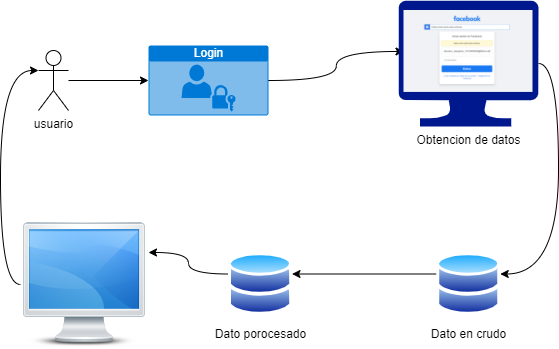
\includegraphics[ scale=0.6]{Imagenes/Fuentes/Idea_inicial.png}
	\caption{Diseño de las fases de la app}
	\label{Idea_inicial}
\end{figure}

\begin{figure}
 	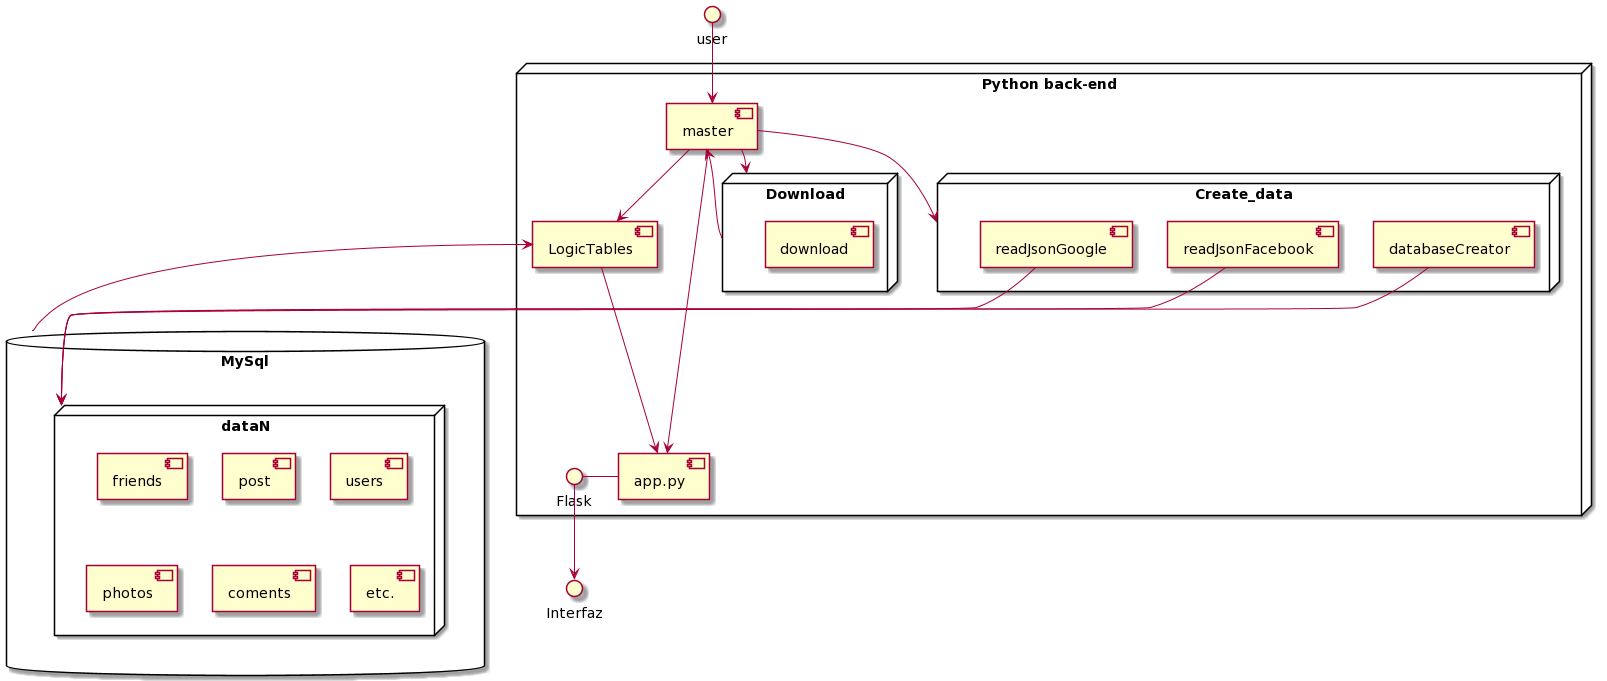
\includegraphics[ scale=0.25]{Imagenes/Fuentes/diagrama_back_end.png}
 	\caption{Diagrama de componentes del back-end}
 	\label{Diagrama_back_end}	
\end{figure}

\begin{figure}
 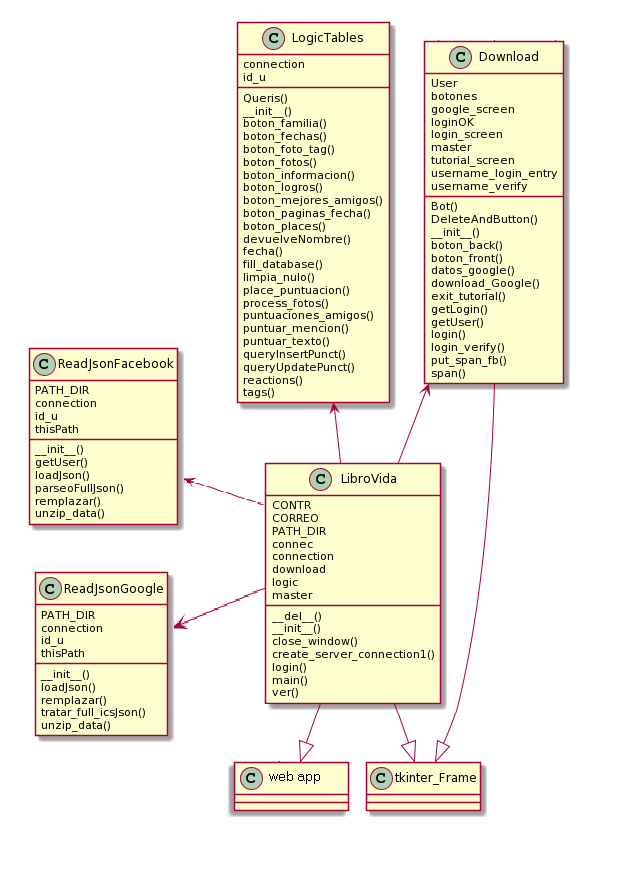
\includegraphics[ scale=0.75]{Imagenes/Fuentes/Diagrama_de_clases_backend.png}
 \caption{Diagrama de clases del back-end de la aplicación}
 \label{Diagrama_clases}
\end{figure}


Para llegar a nuestro objetivo de diseño, hemos dividido la implementación de la aplicación en diferentes módulos, los cuales hemos ido creando siguiendo el diseño inicial. Estos son:

\begin{itemize}
	\item \textbf{ Descarga de datos de Facebook.}
	\item \textbf{ Creación de las tablas, parseo de JSON e inserción.}
	\item \textbf{ Tratamiento de los datos.}
	\item \textbf{ Interfaz de usuario versión 1.}
	\item \textbf{ Descarga y tratamiento de datos de Google.}
	\item \textbf{ Interfaz de usuario versión 2.}
\end{itemize}

En las siguientes secciones  vamos a explicar en más detalle en que constan estas etapas. Para ver el código en detalle, consulta el GitHub del proyecto: 	https://github.com/NILGroup/TFG-2021-RedesSociales 


\section{Descarga de datos de Facebook}

Esta primera parte de la aplicación es la que más ha variado en todo el proceso, aunque empezó siendo un scraper que sacaba todos los datos automáticamente sin interferencia del usuario, las dificultades que pone Facebook a este tipo de técnicas nos obligó a optar por una opción mucho menos potente, pero igual de eficaz. Dividiéndose en las etapas de: Identificación de usuario, Tutorial de descarga y Preparación de carpetas. Todas estas etapas se ven reflejadas en la \textbf{Figura 4.4} donde se muestra el diagrama de Actividad a seguir para descargar los datos. En las siguientes subsecciones definimos también las etapas de este proceso:

\begin{figure}
	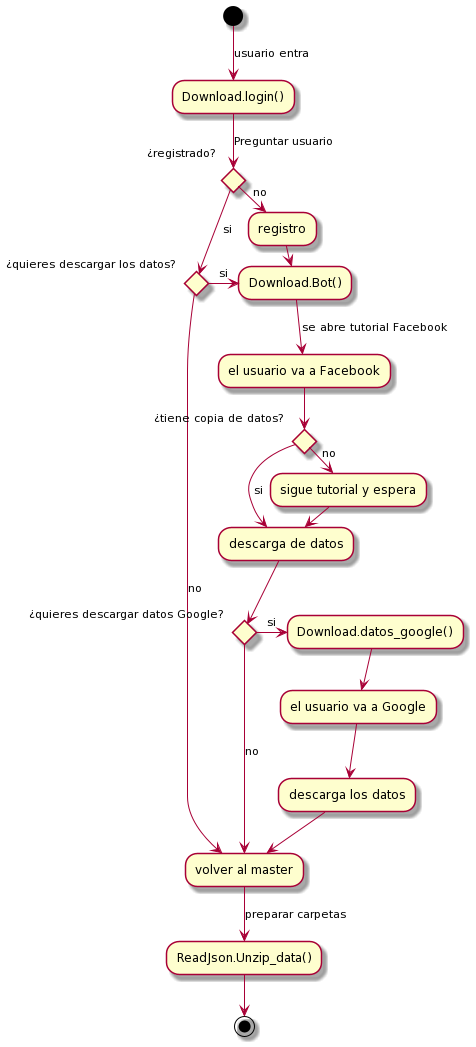
\includegraphics[scale=0.55]{Imagenes/Fuentes/Diagrama_actividad_descarga.png}
	\caption{Diagrama deactividad para la descarga de datos}
	\label{DiagramaDescarga}
\end{figure}


\subsection{Identificación de usuario}
Los datos de Facebook en formato JSON tienen un tamaño considerable, por lo que el tiempo que tarda en proporcionártelos puede variar desde varios minutos a incluso rondar la hora si el usuario es muy activo. Esto hace necesaria una manera de que el usuario decida si volver a descargarlos o no, para esto usamos SQLite3, la base de datos ya explicada en capítulos anteriores y que nos permite almacenar una confirmación de las descargas para cada usuario que haya usado la aplicación. 

La función que domina esta parte de la aplicación es \textbf{login\_verify}, la cual se conecta a la base de datos y comprueba que el usuario no está ya registrado en ella, así como la última vez que ha descargado los datos, para preguntarle si considera necesario volverlos a descargar a través de un span o ventana emergente. 

Los spans se gestionan con funciones auxiliares, que son la función \textbf{span}, la cual genera un pop-up con botones para mostrar información y confirmar pasos. Esta recibe como argumento una lista de los botones necesarios, el título del span, el texto a mostrar y el tamaño de la ventana, devolviendo el botón que se ha pulsado en el span para actuar en consecuencia. Esto lo hace con ayuda de la función \textbf{DeleteAndButton}, que borra el span y avisa del botón pulsado.

Todo esto está gestionado por la función \textbf{login}, que es la principal de la clase, simplemente crea la ventana padre en Tkinter y pregunta el correo del usuario que se utiliza como id. Si el usuario accede a descargar datos, se llama a la última función \textbf{Bot} dentro del tutorial de descarga. En la versión 2, gestionamos los datos de Google a partir de este punto.

\subsection{Descarga de datos}
Manejada por \textbf{Bot} controla toda la función web con Selenium. Empieza borrando los datos existentes en la carpeta de descarga, para evitar datos duplicados o errores si el usuario ha introducido datos externos en ella. A continuación, configura las opciones de Google Chrome para que, entre otras cosas, la descarga se haga automáticamente a la carpeta necesaria y evitar problemas. Después, se manda al usuario a la pantalla de login de Facebook, donde el bot añade directamente el usuario añadido y pide al usuario que añada la contraseña (que en un inicio incluía también el Bot, pero los niveles de seguridad eran menores y decidimos descartarlo). Esta acción redirige al usuario a la carpeta de descarga, donde con la función \textbf{put\_span\_fb}, implementada en JavaScript, se muestra un tutorial en la propia web de Facebook para ayudar al usuario a descargar los datos. Después de todo esto, la función Bot espera a que la carpeta de descarga contenga algún dato y espera un tiempo prudencial para que la descarga se complete, pasando a continuación el control a la fase de preparación de carpetas.

\subsection{Preparación de carpetas}
Una vez con los datos en formato zip en la carpeta adecuada y el navegador cerrado, cosa de la que se ha encargado Selenium, la función \textbf{unzip\_data} del fichero ReadJsonFacebook.py se encarga de tratar esta carpeta y descargar todos sus datos para su utilización en el siguiente módulo de la aplicación, donde se almacenarán estos datos para su tratamiento. \newpage

\section{Creación de las tablas, parseo de JSON e inserción en las tablas}


Una vez realizada la descarga de los datos en formato zip y extraídos los archivos, lo primero que hubo que hacer fue analizar el contenido de estos para ver que datos eran útiles, la carpeta está organizada en distintas subcarpetas (amigos, comentarios, likes, etc.). Estas carpetas contienen los mismos datos ya explicados en el capítulo 3, y cada subcarpeta contiene uno o varios archivos JSON que contiene la información del usuario en ese apartado. Cada una de las subcarpetas que hemos analizado, la hemos trasladado a una o varias tablas en la base de datos. En función de los datos que consideramos útiles dentro de estas carpetas (también explicado en el apartado de datos de Facebook y Google del capítulo 3), íbamos añadiendo los atributos y relaciones de estas tablas. Las etapas de esta sección se pueden ver reflejadas en el diagrama de la figura 4.5.

\begin{figure}
	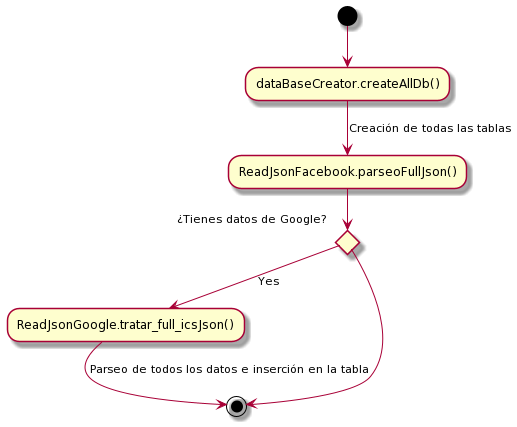
\includegraphics[scale=0.8]{Imagenes/Fuentes/Parseo.png}
	\caption{Diagrama del parseo de datos}
	\label{DiagramaParseo}
\end{figure}

\subsection{Creación de tablas SQL}

Para este apartado, hemos creado una base de datos relacional, la cual queda ilustrada en el diagrama de la \textbf{figura  4.6}, así como en el \textbf{Apéndice A}, donde detallamos todas las tablas con su función, un listado de los diferentes campos y una pequeña descripción de lo que guarda cada uno.

El código perteneciente a esta parte del proyecto se encuentra en el fichero dataBaseCreator.py que se llama cuando el usuario pulsa el botón de ver libro de vida y antes de inicializar el Back-end para poder visualizarlo.

Como vamos a tener que realizar muchas consultas a la base de datos hemos creado dos funciones que nos ahorran líneas de código:

\begin{itemize}
	\item \textbf{ create\_db\_connection}(host\_name, user\_name, user\_password, db\_name): Función que sirve
	para establecer directamente conexión con la base de datos creada (db\_name). Es llamada antes de la creación de las tablas y también antes de hacer inserciones.
	\item \textbf{ execute\_query(connection, query)}: Función que ejecuta la consulta pasada por parámetro en forma de string. Es llamada cada vez que queremos crear una tabla, insertar datos o extraerlos para manipularlos.
	
\end{itemize}

\begin{figure}
	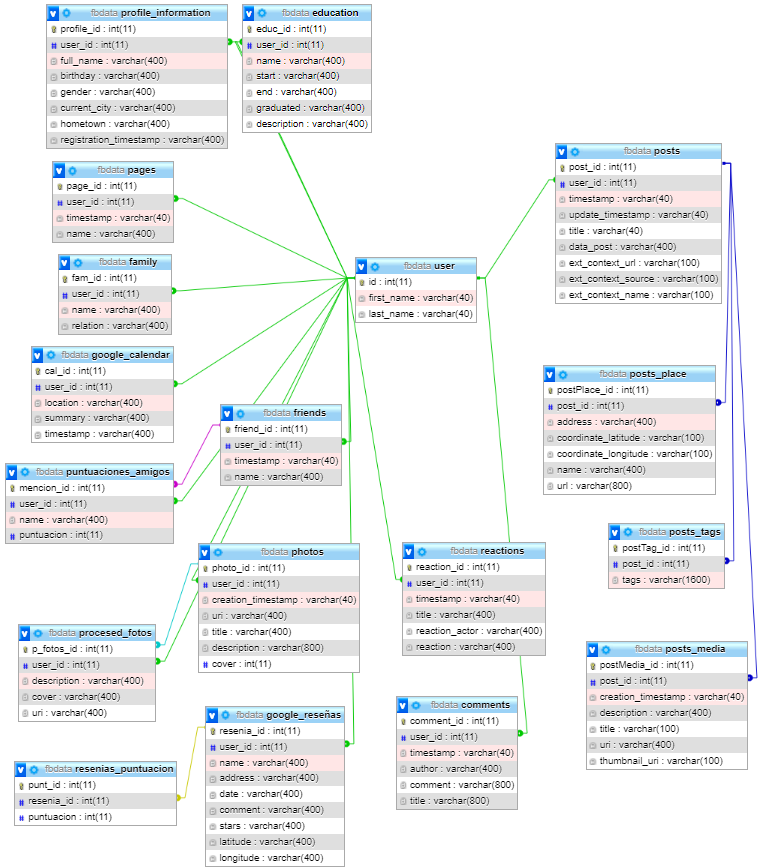
\includegraphics[scale=0.8]{Imagenes/Fuentes/DiagramaBDSQL.png}
	\caption{Diagrama de la Base de Datos}
	\label{DiagramaBDSQL}
\end{figure}
Las tablas de SQL están detalladas en el Apéndice A. 

\subsection{Parseo de JSON e inserción en las tablas}

Para tener los datos del paciente en una base de datos con la que podamos trabajar, primero tenemos que parsear la información del sujeto en cuestión, que viene en formato JSON, ICS, CSV. Esto es, clarificarla y dejarla en un formato que pueda ser leído por las tablas SQL.

JSON (acrónimo de JavaScript Object Notation, «notación de objeto de JavaScript») es un formato de texto sencillo para el intercambio de datos.
ICS es la extensión de los archivos del estándar ICalendar para el intercambio de información de calendarios. Ya que el calendario de Google viene en este formato vamos a transformar a formato JSON para poder tratarla más fácilmente. 
Todo el código perteneciente a esta parte del proyecto se encuentra en los ficheros ReadJsonFacebook.py y ReadJsonGoogle.py.

En esta parte hemos creado también algunas funciones que nos ahorran líneas de código, como por ejemplo:
\begin{itemize}
	\item loadJson(selef, path): esta función recibe por parámetro la ruta de un fichero JSON el cual descodifica, y devuelve una variable con la que se puede empezar a trabajar en Python.
	\item remplazar(self, s): esta función recibe por parámetro un String y lo escapa para que a la hora de insertarlo en la consulta SQL no de problemas.	
\end{itemize}

Para entender mejor esta parte, vamos a describir los distintos ficheros JSON que  hemos tratado dentro de la carpeta de Facebook y como se corresponden esos datos con las tablas de la base de datos.
\begin{itemize}
	\item friends.json: Este fichero está formado por un array en el que cada elemento hace referencia a un amigo del usuario en Facebook, cada elemento está formado por una estructura en la que se define el timestamp(la fecha en formato Facebook) de cuando se hicieron amigos, así como el nombre y apellidos del amigo. Estos datos los recogemos y los guardamos en la tabla fbdata.friends.
	
	\item comments.json: Este fichero también está formado por un array en el que cada elemento es un comentario. Cada elemento está compuesto por una estructura formada por el timestamp, el título del comentario y otra estructura en la que se definen el autor y el contenido del comentario. Estos datos son almacenados en la tabla fbdata.comments.
	
	\item posts\_and\_comments.json: En este fichero se guardan los likes y reacciones del usuario, es también un array en el que en cada elemento se describe el like o reacción del usuario a través de una estructura compuesta por el timestamp, el título(en el que se describe el destinatario al que se le está dando el like) y una estructura formada por el tipo de reacción y el actor de la misma. Guardamos estos datos en la tabla fbdata.reactions.
	
	\item profile\_information.json: Este fichero es algo más complejo, de aquí se obtiene información que va a distintas tablas. El fichero define una estructura con los campos:
	\begin{itemize}
		\item name: es una estructura formada por el nombre y los apellidos del usuario.
		
		\item birthday: es una estructura compuesta por el día, el mes y el año de nacimiento del usuario.
		
		\item gender: define el género del usuario.
		
		\item current\_city: es una estructura que define el lugar donde vive ahora mismo el usuario y un timestamp que define desde cuando.
		
		\item hometown: otra estructura más formada por el lugar de nacimiento del paciente y un timestamp que define cuanto tiempo vivió allí.
		
		\item registration\_time: Es un timestamp con la fecha de registro del usuario en Facebook.
	\end{itemize}

	Todos los datos mencionados de profile\_information hasta aquí, se guardan en la tabla fbdata.profile\_information.
		
	\begin{itemize}
		\item family\_members: Es un array en el que cada elemento define una estructura para representar a un familiar del usuario, esta estructura se compone del nombre y apellidos del familiar, la relación parental que hay entre ellos y el timestamp que representa desde cuando son amigos en Facebook. Estos datos se guardan en la tabla fbdata.family.
		
		\item education\_experiences: Es un array donde los elementos que lo componen representan las distintas formaciones educativas del usuario. Cada elemento está constituido por una estructura con campos para definir el nombre del lugar de estudios, la fecha de inicio, la fecha de fin y si está graduado o no. Estos datos se almacenan en fbdata.education.
		
		\item work\_experience: También es un array en el que cada elemento representa un lugar de trabajo. Este lugar de trabajo se define a través de una estructura con el nombre del trabajo, la descripción de lo que se hacía en su trabajo y las fechas de inicio y fin. Al ser muy parecido a education\_experience, hemos añadido estos datos en la tabla fbdata.education.
		
	\end{itemize}

		\item pages.json: Es un array en el que cada elemento describe una página a la que el usuario ha dado like. Cada elemento se compone de una estructura con el nombre de la página y la fecha en la que se empezó a seguir ese contenido. El contenido de este fichero se almacena en la tabla fbdata.pages.
	
		\item Fotos de Facebook: Al tener Facebook la posibilidad de guardar las fotos en álbumes, tenemos una carpeta llamada álbum en la que se almacena un archivo JSON para cada uno de los distintos álbumes del usuario, por lo que recorreremos todos los JSON que haya en la carpeta para ir recopilando en la tabla fbdata.photos todas las fotos que haya subido el usuario a Facebook. Cada fichero JSON está compuesto por una estructura con el nombre del álbum y un array con las fotos de ese álbum. Este array de fotos está formado por elementos en los que en cada uno hay una estructura para detallar toda la información de la foto, estos campos son la ruta donde está guardada la foto, el título de la foto, la descripción, la fecha de subida y si es portada o no.
	
		\item your\_post.json: Este fichero está también formado por un array en el que los elementos contienen la información de cada post a través de una estructura. Los campos de esta estructura son la fecha de publicación del post, el título, la descripción, la url externa que se halla compartido en ese post, el nombre del contenido externo unido a este post, un array con los archivos adjuntos (fotos y ubicaciones), y un array con las personas etiquetadas en la publicación. Excepto los archivos adjuntos y las etiquetas se almacena todo fbdata.posts.
	
		Los archivos adjuntos están formados por una estructura con un campo para guardar las fotos y otro para guardar las ubicaciones. El campo para guardar las fotos está formado por un array con todas las fotos adjuntadas al post, cada una se compone de una estructura con los campos título de la foto, descripción, ruta de la foto y la fecha de subida de la foto. Las distintas fotos se guardan en la tabla fbdata.post\_media con una foreign key que hace referencia al post al que pertenecen.
		
		Las ubicaciones son similares, pero guardan los campos dirección, latitud, longitud, nombre de la ubicación y una url a la página de Facebook para esa ubicación. Estas se guardan en una tabla llamada fbdata.posts\_place con una foreign key que hace referencia al post al que pertenecen.
		
		Las etiquetas son un array en el que cada elemento es el nombre y apellidos del amigo de Facebook que está etiquetado. Se guardan en la tabla fbdata.posts\_tags con una foreign key al post al que pertenecen.
	
\end{itemize}


El proceso de parseo es similar para los distintos archivos JSON. Primero se carga con la función loadJson() el contenido del fichero JSON en una variable que nos permita trabajar los datos, después se recorre esta variable con uno o varios bucles, según las profundidades que tenga y se guardan los datos en variables tras ser scapeadas con la función remplazar, para su posterior inserción en la base de datos.
Para la inserción se guardan en variables de tipo String las consultas que serán ejecutadas con la función execute\_query junto a los datos escapados mencionados anteriormente. 

Con esto, los datos del usuario ya estarían a salvo en la base de datos y listos para tratar, de lo cual se encargara la siguiente etapa.

\section{Tratamiento de los datos}

La implementación de esta sección del proyecto se encuentra en el fichero LogicTables.py, y se encarga de recolectar todos los datos almacenados en la BBDD y tratarlos para conseguir un formato entendible y mostrable al usuario. Se divide en esas dos partes: ``extracción y tratamiento de datos'' y ``Envió de datos a la interfaz gráfica de usuario''. Estas últimas tienen la peculiaridad de ser funciones botón, porque se llaman así en la interfaz (boton\_accion). Se puede ver las etapas de esta sección en el diagrama de la \textbf{figura 4.7.}

A continuación detallaremos las dos partes.
\begin{figure}
	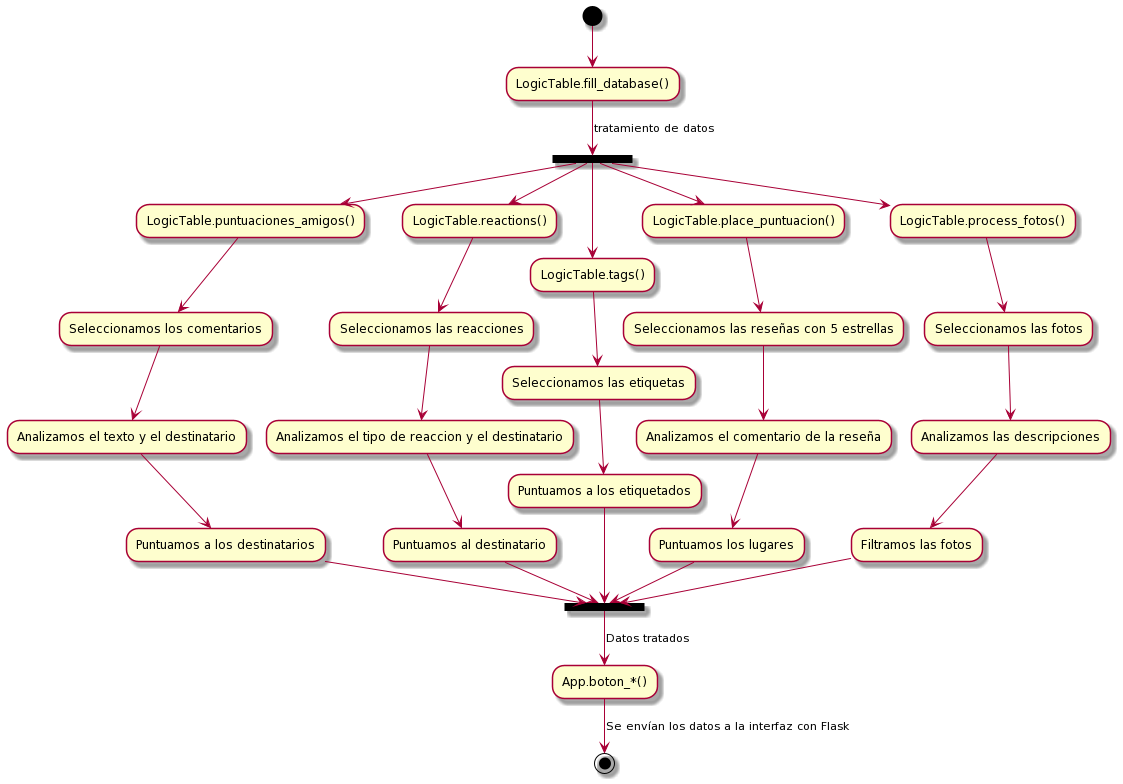
\includegraphics[scale=0.33]{Imagenes/Fuentes/tratamiento.png}
	\caption{Diagrama del tratamiento de datos}
	\label{DiagramaTratamiento}
\end{figure}
 
\subsection{Tratamiento}
Además de buscar un formato entendible y mostrable, en esta parte queremos darle un sentido extra a los datos, para ello hemos clasificado los comentarios, las reacciones y likes, y los amigos etiquetados del usuario, para darles una puntuación en \textit{puntuaciones\_amigos}, clasificando así los más importantes para el usuario. También hemos cruzado datos de diferentes partes, como tags o menciones, para añadir más valor a las fotos, o, en la segunda versión, datos de Google con datos Facebook.

\begin{itemize}
	\item Para clasificar los comentarios recorreremos la tabla con un bucle e iremos obteniendo la persona o página a la que va dirigida el comentario por parte del usuario. Para ello nos apoyaremos de la función devuelveNombre() que hemos creado, la cual recibe por parámetro el comentario en tipo string y calcula los caracteres que ocupa el nombre de la persona que publica el comentario, más los caracteres que ocupa el tipo de comentario (ha comentado la publicación de…, ha respondido al comentario de…, ha comentado la foto de…, ha comentado el vídeo de…, ha comentado el enlace de…, etc.) y finalmente recortar el string para devolver el nombre de la persona o página a la que va dirigido.
	Una vez obtenido el nombre, si no existe un registro de esta persona en la tabla de \textit{puntuaciones\_amigos} lo insertamos con la puntuación a uno, y si ya existe le sumaremos uno a la puntuación que ya tenga calculada.
	
	\item Para clasificar los likes y las reacciones seguiremos un procedimiento parecido al descrito en el apartado anterior. Recorremos la tabla \textit{reactions} y recortaremos el string del campo \textit{title} para obtener el usuario al que va dirigido la reacción, también seleccionaremos el campo \textit{reaction} en el que se guarda el tipo de reacción y en función a esta, daremos más o menos puntuación en la tabla \textit{puntuaciones\_amigos} a los amigos o páginas involucradas. A continuación se muestra el valor que se le otorga al tipo de reacción:
	\begin{itemize}
		\item LIKE: 1 punto.
		\item LOVE: 3 puntos.
		\item JAJA: 2 puntos.
		\item WOW: 1 punto.
		\item SAD: -2 puntos.
		\item ANGRY: -2 puntos.
	\end{itemize}

	\item Hemos considerado que las personas que salen etiquetadas en las fotos del paciente, por norma general tienen un vínculo importante con este. Por lo que hemos recorrido la tabla \textit{posts\_tags} con un bucle, y con ayuda de la función \textit{eval()} del estándar de Python, convertimos en un array el campo \textit{tags}, donde Facebook almacena a las personas etiquetadas en formato de string. Después, recorremos este array de amigos para darles una puntuación en la tabla \textit{puntuaciones\_amigos}.
	
	\item Otra parte importante del tratamiento es la utilización de un sistema de procesamiento del lenguaje(NLP) para la valoración de las emociones en los textos que hay dentro de toda la aplicación, hemos creado una función puntuar\_texto, la cual limpia el texto, eliminando las posibles interferencias, quitando mayúsculas, números, o algunos símbolos que no se pueden analizar, mientras que mantenemos otros símbolos o emoticonos. Después traduce el texto al inglés, puesto que en español (como ya hemos mencionado en el capítulo 2) no hay, de momento, herramientas de NPL tan avanzadas como nos gustaría. Por último, lo pasamos por el analizador de sentimientos, que devuelve una puntuación en función de los sentimientos detectados en el texto.
	
	Estos textos analizados nos han sido de gran utilidad en varias partes de la aplicación, ya que nos han permitido evaluar que lugares han sido importantes, que comentarios son los positivos y por lo tanto quienes son los amigos con los que te relacionas más positivamente y otras muchas cosas.

\end{itemize}

\subsection{Envió de datos a la interfaz}
Esta parte se centra en la organización de los datos ya tratados y almacenados en SQL, los selecciona con diferentes querys para entrelazar los que están relacionados entre ellos y sacar el máximo partido a los mismos. Hemos separado el código en las funciones que posteriormente se llamaran en la GUI. Estas funciones son:

\begin{itemize}
	\item \textbf{boton\_amigos\_fecha:} Analiza tus 10 mejores puntuaciones entre los amigos que tiene el usuario y devuelve la fecha en la que conoció a esos amigos en la red social en formato JSON: (`fecha': YYY-MM-DD HH:MM, `amigo': nombre, `puntuación': entero). Esta función lee de las tablas friends y puntuaciones\_amigos.
	
	\item \textbf{boton\_paginas\_fecha:} Analiza tus 10 mejores páginas entre las que el usuario es miembro y devuelve la fecha en la que conociste a tus amigos en formato JSON: (`fecha': YYY-MM-DD HH:MM, `página': nombre de página, `puntuación': entero). Esta función lee de las tablas friends y puntuaciones\_amigos.
	
	\item \textbf{boton\_places:} Analiza todos los lugares visitados por el usuario en Facebook y Google devolviendo un JSON con el formato: (`fecha': YYY-MM-DD HH:MM, `contenido': contenido del post, `url': url al contenido del post, `donde': dirección del lugar, `personas\_list': array de personas con las que apareces, `fotos\_list': array de fotos del lugar, `coordenadas': coordenadas para buscar en Google y `puntuación': puntuación que le hemos dado al lugar según la interacción de usuario). Esta función lee de la tabla post\_places, resenias\_puntuacion y google\_reseñas.
	
	\item \textbf{boton\_foto\_tag:} Analiza la lista de mejores amigos (puntuación) y manda la URI de los archivos en local que apunta a esas fotos, en las que el usuario aparece con sus mejores amigos, devolviendo: (`amigo': nombre, `fotos\_list': array de fotos, `fecha': YYY-MM-DD HH:MM). Esta función lee de las tablas friends y puntuaciones\_amigos, posts\_tags y post\_media.
	
	\item \textbf{boton\_fotos:} Analiza las fotos de portada, que consideramos importantes o con descripción positiva (a través de NLP) y devuelve la URI de los archivos en local que apunta a esas fotos y si son o no portada, devolviendo (`cover': si es cover o no, `URI': URI a la foto). Esta función lee de la tabla profile\_information.
	
	\item \textbf{boton\_informacion:} devuelve la información básica del usuario: (`nombre': nombre, `cumple': YYY/MM/DD, `género': género, `vivienda actual': vivienda actual,`lugar de nacimiento': lugar de nacimiento, `inicio de los datos': inicio de los datos). Esta función lee de la tabla family.
	
	\item \textbf{boton\_familia:}Devuelve la información de tu familia: (`nombre': nombre del familiar, `relación': relación de parentesco)
	\item \textbf{boton\_logros:} Devuelve tu información académica y laboral: (`nombre': nombre, `inicio': fecha de inicio del curso, `fin': fecha de fin del curso, `graduado': si el usuario está graduado). Esta función lee de la tabla education.
	
	\item \textbf{boton\_fechas:} Devuelve las fechas importantes del programa con todas las actividades que has realizado en ellas, cogiendo datos de varias tablas:
	\begin{itemize}
		\item Facebook Friends: Coge el timestamp de cuando te has hecho amigo de los 50 mejores amigos que tienes según nuestra puntuación calculada.
		\item Google calendar: Coge el timestamp de los eventos importantes que has guardado en Google.
		\item Google reseñas: Coge el timestamp de cuando has visitado los lugares que has añadido a favoritos.  
		\item Facebook Post media: Coge el timestamp de cuando has subido, o has sido etiquetado en fotos importantes.
	\end{itemize}

\end{itemize}

Esta parte de la aplicación tiene el punto fuerte de unir una gran cantidad de datos, como los de la función que trata los post o los amigos, resumiéndolos en unos pocos datos importantes mucho más fáciles de manejar, o mezclando datos de diferentes fuentes como los datos de todas las fechas de Google y Facebook. Estos datos en el formato manejable son los que se pasan a la interfaz de usuario para que se muestren, lo cual detallamos en el siguiente apartado

\section{Interfaz de usuario versión 1.}

Esta parte de la aplicación estaba comandada por la clase VistaLibroVida() y master() principalmente, en el archivo showLifeBook.py y master.py, se trataba de la parte que implementaba una vista de usuario en tkinter, pero que finalmente fue descartada por diversas razones, entre ellas la dificultad de crear tablas, imágenes y libros de vida en general, con las librerías que proporcionaba tkinter. Utilizábamos principalmente las siguientes:

	\begin{itemize}  
		\item ttk: que proporciona acceso a un conjunto de widgets para mejorar el estilo de tkinter y poder definir objetos como treeview, que es el elemento que utilizábamos para la visualización de tablas, pero que está pensado más como un sistema de archivos.
		
		\item tkFont: que sirve para manejar fuentes en tkinter y lo utilizábamos para cambiar el tamaño o fuente de las letras en partes como el título o la sección en la que se encuentra el usuario.
		
		\item PIL: Es una librería gratuita que permite la edición de imágenes directamente desde Python. Soporta una variedad de formatos, incluidos los más utilizados como GIF, JPEG y PNG. La utilizábamos para mostrar las fotos del paciente, pero tenía problemas al mostrar fotos, enlaces y estilos, por lo que decidimos descartarlo en pos de la aplicación web mucho más amigable que tenemos en la versión actual.
		
	\end{itemize}
		Empezamos por máster, que es la clase que controla el resto de la aplicación, siendo la que posteriormente se puede convertir en un ejecutable de Windows con ``pyinstaller''. Esta empieza creando la ventana raíz de la que heredan el resto de ventanas y preguntado al usuario que acción quiere realizar, estando disponibles las acciones de ``Login'', ``Crear datos'' y ``Ver libro de vida'', llamando estas a las respectivas clases que realizan la funcionalidad que describe el botón que se pulsa.
		
		También comprueba que los datos estén disponibles antes de pasar a la siguiente función y se encarga de destruir la aplicación si el usuario cierra la ventana. Esta parte se ha mantenido en la segunda versión de la interfaz, así como la parte de descarga de datos, que ya fue explicada con más detalle en las librerías del capítulo 3. Se han mantenido porque necesitábamos una interfaz Python para tratar y descargar los datos, ya que las librerías y funciones principales estaban escritas en Python, por lo que decidimos no migrarla a React.

A partir de aquí, se descartó todo por la dificultad de crear un libro de vida con Tkinter, es decir, la parte de visualización de datos. Esta parte implementaba una vista de usuario para mostrar los datos ya tratados y formateados. Decidimos centrarnos en la utilización de botones Tkinter para que el usuario seleccione la vista que le interesa, y si esa vista tiene fotos o enlaces externos, el usuario puede seleccionar cuál visualizar por medio de otro botón. 

Mientras que el resto de la GUI está gestionada por el formato pack() de tkinter, esta parte seguía el formato grid(), el cual era más conveniente para la creación de tablas y colocación de objetos en diferentes partes de la ventana. El formato está gestionado por filas y columnas, en las que habíamos colocado los 8 botones para las diferentes posibilidades que tenía el usuario, una tabla que muestra los datos seleccionados y, por último, unos botones de selección para enlaces externos que puedan aparecer en los datos. Para cada sección que puede elegir el usuario, se había definido una función para coger el evento de botón y realizar la acción correspondiente, así como una variable que guardaba los datos para evitar cargas necesarias. Después, se enviaban estos datos a la función principal de Python create\_table(), que gestionaba toda la parte de borrar datos anteriores para que no se pisaran y separaba el diccionario para mostrarlo como tabla, mostrando desplegables si los datos contienen una lista como puede ser una lista de fotos dentro de un mismo post o una lista de amigos etiquetados en la misma foto.

Todo esto fue descartado por la dificultad de mostrar fotos y por la apariencia más bien primitiva de la app, la cual no nos convenció del todo y creíamos que tenía mucho margen de mejora. En la siguiente figura (4.8) se puede ver como era la interfaz antes del cambio de tecnología.

\begin{figure}
	\begin{center}
		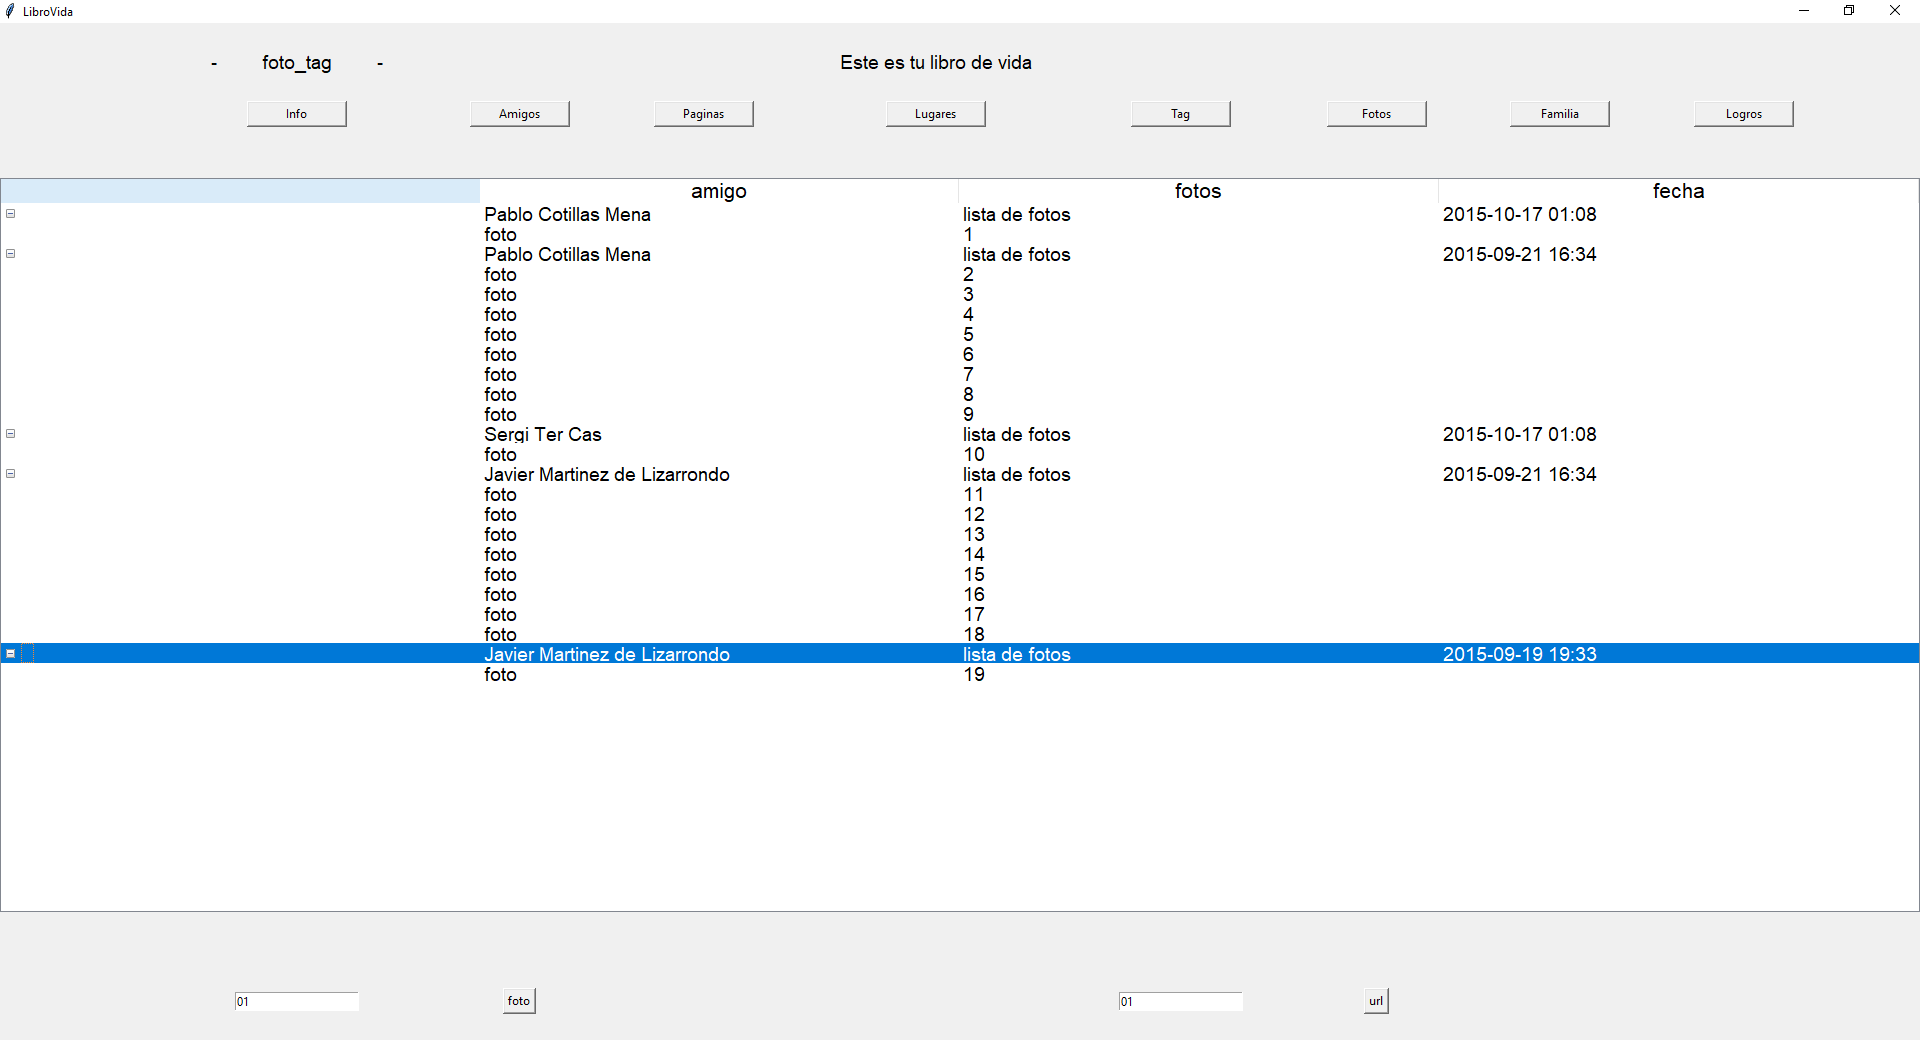
\includegraphics[scale=0.25]{Imagenes/Fuentes/tablasFoto.png} 
		\caption{Tabla de la antigua interfaz}
		\label{Tinicial}
	\end{center}
\end{figure}
\newpage
 
\section{Descarga de datos de Google}


Una vez tuvimos una aplicación funcional con los datos de Facebook, creímos oportuno ampliarlos con los datos que almacena otra gran empresa, como lo es Google. Esto lo hicimos porque, aunque Facebook es la red social más utilizada, es posible que no todo el mundo tenga una cuenta, sin embargo es más probable que un paciente haya utilizado alguna vez Google Maps, o haya guardado sus fotos en aplicaciones como Google Fotos, que en este momento viene preinstalada en los móviles Android, ya que los móviles sí que son un elemento prácticamente extendido a toda la población.

Estos datos también nos acarrearon problemas, pues Google protege aún más sus datos frente al scraping, ni siquiera es posible registrarse en Google si estás entrando con un bot que simule a un humano o un navegador automatizado, por lo que hemos delegado completamente la descarga de los datos de Google al usuario de la aplicación, eso si, con un tutorial de ayuda escrito en Tkinter e integrado en nuestra propia aplicación para que esto sea lo más sencillo posible.

Esta parte, de manera similar a los datos de Facebook, se caracteriza por una descarga basada en un tutorial y la preparación de la carpeta, saltándose el paso de login pues el usuario en este punto ya debería estar registrado en la aplicación, pero al obtener nuevos datos, también consta de una parte en la que estos datos se tratan y analizan.

\subsection{Tutorial de descarga y preparación}

Al no poder controlar todas las funciones web con Selenium, no podemos configurar las opciones de Chrome para que la descarga se haga automáticamente a la carpeta necesaria, pero Tkinter si deja abrir navegadores web, por lo que lo primero que se hace es mandar al usuario a la página de Google Takeout, donde se puede descargar sus datos una vez se registre con su cuenta principal de Google. Después la función datos\_google se encarga de mostrar el tutorial de Tkinter con todos los pasos a seguir por el usuario para descargarse sus datos. Hacemos hincapié en que se guarden en la carpeta descargas, pues no somos capaces de adivinar donde se ha descargado la carpeta de manera simple.

Una vez con los datos en formato ZIP en la carpeta de descargas, la función \textbf{unzip\_data} del fichero ReadJsonGoogle.py se encarga de tratar esta carpeta y descargar todos sus datos para su utilización en el resto de la aplicación, donde pasará por las mismas etapas que los datos de Facebook, se almacenarán para su tratamiento, se tratarán y posteriormente se mostrarán por la nueva GUI. Al haber realizado una aplicación escalable, la cantidad de cambios a realizar con estos nuevos datos no nos ha supuesto una modificación en ninguna parte fundamental del código, solamente añadir las funciones que tratan y analizan los nuevos datos, juntándolos con los de Facebook, así como la inserción de los nuevos JSON en la base de datos

Esta carpeta está compuesta de los datos mencionados en el capítulo 3 donde ya hemos explicado cuáles consideramos útiles, pero vamos a detallar un poco la estructura de los ficheros JSON, ICS y CSV y la correspondencia con las tablas de la base de datos.
\begin{itemize}
	\item user\_name.ics: Este fichero lo convertimos en JSON gracias a la librería Jicson, que nos genera un array en el que cada elemento corresponde con un evento en el calendario formado por una estructura con la fecha de comienzo del evento, la fecha de fin, la localización, y la descripción. Estos datos son almacenados en la tabla fbdata.google\_calendar.
	
	\item reseñas.json: Este fichero se define a través de un array en el que cada elemento haca alusión a una reseña que haya publicado el usuario sobre algún establecimiento. Cada elemento se compone de una estructura en la que el campo ``geometría'' representa un lugar, que se almacena como la latitud y longitud de este, el campo de la localización es también otra estructura que almacena la URL a Google\_maps, con la dirección del establecimiento y el nombre del mismo, y por último los campos en los que se almacenan el comentario que se escribió y el número de estrellas con las que se puntuó al sitio. Estos datos se almacenan en la tabla fbdata.google\_reseñas.
	
	\item Para cada foto de Google, hay un archivo JSON en el que se describen la URL, el título, la descripción y el timestamp de la foto, hemos implementado una función que recorre todo el directorio donde están contenidas las fotos y los JSON para recopilar los datos y almacenarlos en la tabla fbdata.photos.
	
	\item sitios\_favoritos.csv: Cada fila de este fichero referencia a un lugar o establecimiento marcado como favorito por el usuario y cada fila está formada por tres columnas que representan el nombre del lugar, el comentario que se dejó del mismo y la URL. Estos datos son también almacenados en la tabla fbdata.google\_reseñas.
	
\end{itemize}


\subsection{Tratamiento y revalorización de los datos}
Aunque ya hemos definido los datos que hemos elegido en el capítulo 3, aquí vamos a hacer un análisis más detallado de lo que hemos actualizado en la implementación del proyecto para tratar y analizar los datos, así como el valor que estos datos han aportado a los que ya teníamos en la versión anterior. Como ya hemos dicho, la modularidad de la aplicación nos ha permitido modificar los datos sin cambios sustanciales, todo lo que hemos realizado han sido ampliaciones de los datos.

El primero ha sido la incorporación de las fotos que el usuario tenía en Google, para esto hemos analizado las que el usuario ha guardado como favoritas únicamente, pues la cantidad de fotos que un usuario puede tener en sus archivos es enorme, y también hemos cogido las que el usuario ha guardado como fotos de perfil. Estas fotos las hemos añadido a las que ya tenían de Facebook para mostrar.

El segundo ha sido la creación de una organización por fechas de la que aún no disponíamos, pues los datos del calendario de Google han dado más importancia a este apartado. De Google hemos analizado todos los datos del calendario, así como las fechas en las que según Google el usuario estaba visitando lugares que le resultaron importantes. Estos datos los hemos mezclado con diversos datos de Facebook que ya tenían fechas para crear una visualización ordenada como si fuera un timeline, lo cual es un gran aporte para un libro de vida.

El último ha sido la ampliación de los lugares que ya teníamos de Facebook, puesto que Google Maps guarda una gran cantidad de lugares que el usuario ha visitado y reseñas de los mismos que este ha publicado, hay una gran cantidad de datos que se pueden extraer. Hemos cogido las reseñas de los sitios que ha visitado con la mayor puntuación y pasando el texto de la reseña por nuestro analizador de emociones para guardar en una nueva tabla resenias\_puntuacion las reseñas más importantes, y por lo tanto, los lugares que más le han gustado. También los sitios que el usuario ha guardado en favoritos, pues hemos considerado que son los importantes para él. Todo esto se une con los mismos campos que los que tienen los lugares en Facebook, creando así una cantidad de datos de sitios de usuario muy considerable.

\newpage
\section{Interfaz de usuario versión 2}
En este apartado vamos a explicar las cuestiones técnicas de la implementación de la segunda versión de la interfaz, la cual es una aplicación web, y de la cual se pueden ver ejemplos en las figuras 4.10 y 4.11, además de ser explicada con todo lujo de detalle en el \textbf{apéndice B}, donde hay una guía paso a paso con todas las pantallas que tiene nuestra aplicación.


Teniendo en cuanta la cantidad de problemas que tuvimos con la versión 1 de la interfaz y la utilización de Tkinter para la creación de libros de vida, decidimos investigar más a fondo las posibles tecnologías que nos permitían mostrar los datos de la forma más eficiente y fácil de visualizar para el usuario. Entre las diferentes tecnologías que encontramos, como aplicaciones de escritorio en otros lenguajes, o aplicaciones web, nos acabamos decantando por utilizar una interfaz web con dos partes, un back-end en Python, que potenciado con la librería de Flask tratara los datos y los enviara, con un front-end en React que mostrara todo el contenido de una manera fácil y amigable. Esta parte del front-end queda diseñada en la \textbf{Figura 4.9}.


\begin{figure}
	\begin{center}
		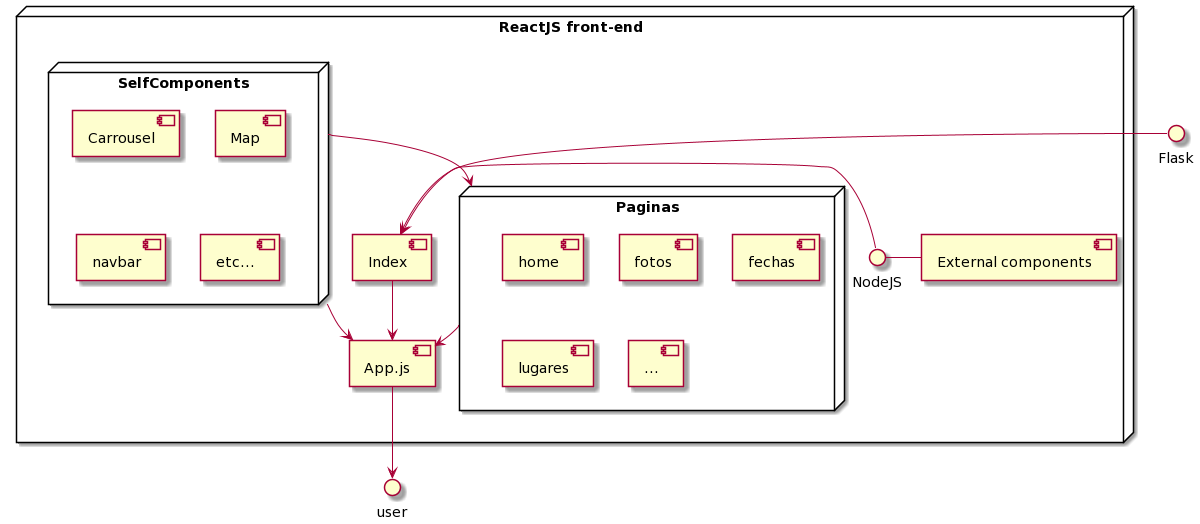
\includegraphics[scale=0.33]{Imagenes/Fuentes/diagrama_front_end.png} \caption{Diagrama con los componentes del front}
		\label{Diagrama_backend}
	\end{center}
\end{figure}



Para la parte del back-end programada en Flask, que funciona creando un archivo app.py que define las rutas de la aplicación de las que luego va a leer React, es decir, la parte del Front. Cada ruta llama a una de las ``funciones botón'' definidas posteriormente en LogicTables y que ya envían los datos en un formato fácilmente transmitible, por lo que lo único que tuvimos que hacer fue crear el enlace entre las dos partes y configurar los puertos. Con todo configurado, la aplicación de React ya tendrá los datos de las páginas si la parte del Back-end esta levantada.

Para la parte del front-end, React ofrece una gran variedad de componentes, un componente es un elemento software visual, independiente y reutilizable, que tiene su propio estado, recibe unas propiedades e implementa su propia lógica de renderizado. El esqueleto principal de nuestra interfaz consiste en un componente principal Navbar, que es una barra de navegación en formato menú que permite al usuario navegar entre las distintas páginas de las que está compuesta la aplicación, las cuales también se renderizan en sus propios componentes, y luego cada una llama a los elementos visuales más simples, es decir, otros componentes (como mapas, carruseles de galerías...) Cada una de estas páginas finales, se corresponde con los datos proporcionados por cada una de las funciones botón, y también hay una página de Home para recibir al usuario y contarle un poco como funciona la web.

\begin{figure}
	\begin{center}
		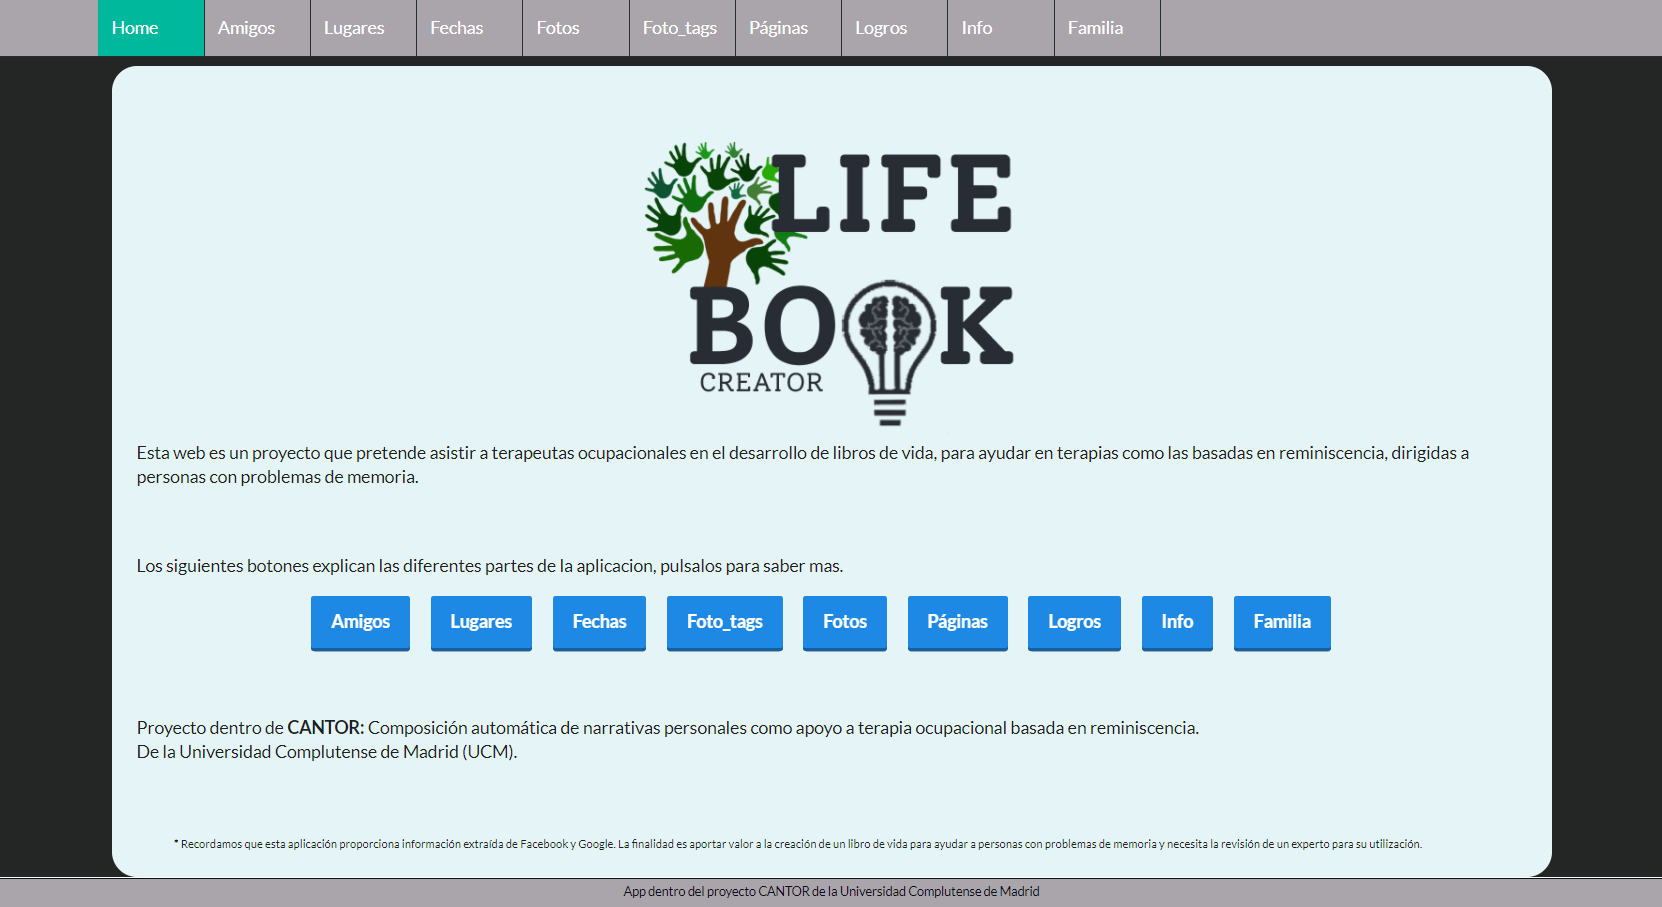
\includegraphics[scale=0.3]{Imagenes/Fuentes/InterfazHome.png} \caption{Interfaz de usuario, apartado de Página principal}
		\label{WebAplication1_4}
	\end{center}
\end{figure}
\begin{figure}
	\begin{center}
		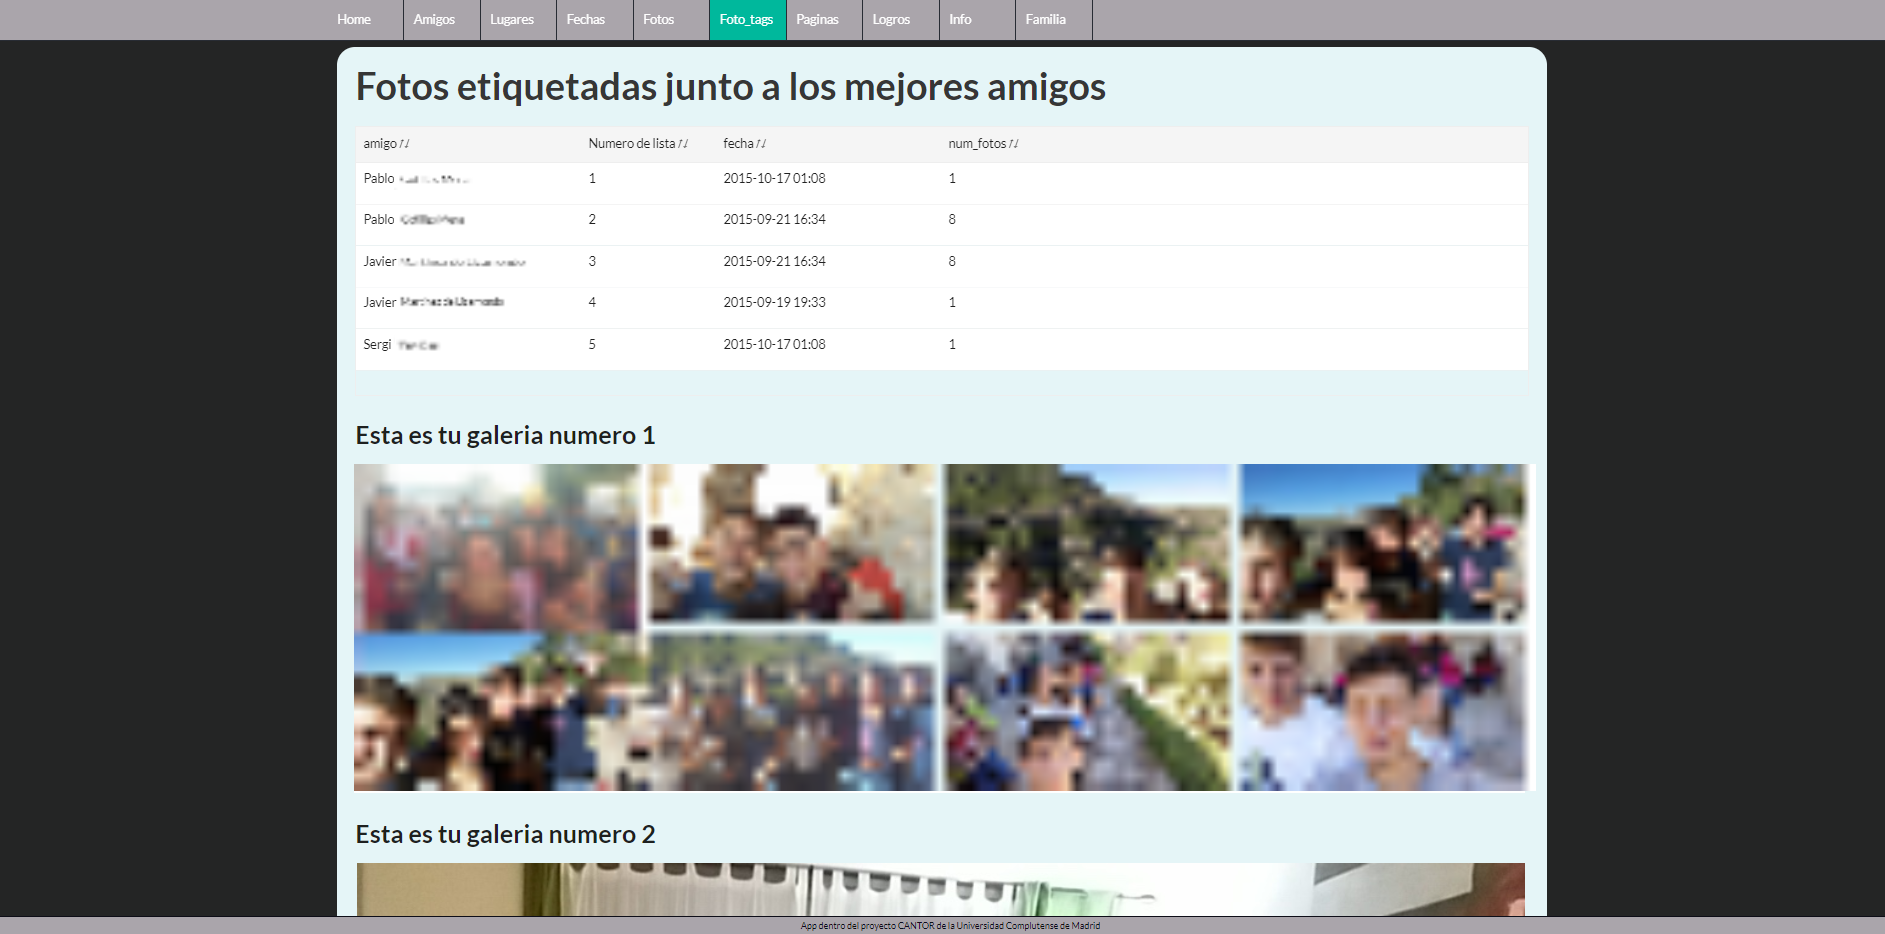
\includegraphics[scale=0.3]{Imagenes/Fuentes/InterfazFoto_tag.png} \caption{Interfaz de usuario, apartado de fotos}
		\label{WebAplication7_4}
	\end{center}
\end{figure}
